\chapter{COMSOL Model Development Workflow}

\section{COMSOL Multiphysics Framework}

COMSOL Multiphysics is a finite-element platform for solving coupled partial
differential equations on a shared geometry. In this work, the Semiconductor
interface solves electronic drift-diffusion and Poisson electrostatics, a
user-defined PDE solves mobile-ion transport, additional PDE or global states
represent degradation, and the Electrical Circuit interface represents lumped
series and shunt pathways. This organization keeps the conservation laws,
domain selections, boundary conditions, and coupling variables inspectable.

\section{Device Stack and Geometry}

The COMSOL model is organized around a one-dimensional PSC stack through the
layer-thickness direction. The physical laboratory architecture, listed from
the illuminated side, is
\begin{equation}
\mathrm{glass}/\mathrm{ITO}/\mathrm{NiO}_x/
\mathrm{MeO\mbox{-}2PACz}/\mathrm{MHP}/
\mathrm{C}_{60}/\mathrm{BCP}/\mathrm{Ag}/
\mathrm{UV\ resin}/\mathrm{glass}.
\end{equation}
The reduced active-device model is
\begin{equation}
\mathrm{ITO}/(\mathrm{NiO}_x+\mathrm{MeO\mbox{-}2PACz})/
\mathrm{Cs}_{0.2}\mathrm{FA}_{0.8}\mathrm{PbI}_3/
(\mathrm{C}_{60}+\mathrm{BCP})/\mathrm{Ag}.
\end{equation}

\begin{table}[H]
\centering
\caption{Laboratory architecture and reduced COMSOL representation.}
\label{tab:lab_comsol_stack}
\begin{tabular}{
>{\raggedright\arraybackslash}p{0.29\textwidth}
>{\raggedright\arraybackslash}p{0.23\textwidth}
>{\raggedright\arraybackslash}p{0.36\textwidth}}
\toprule
Laboratory layer & Nominal thickness & COMSOL treatment \\
\midrule
Front glass & substrate & omitted from electronic domain; defines illumination side \\
ITO & transparent electrode & electrical boundary contact at $x=0$ \\
NiO$_x$ & approximately 30 nm & combined into 35 nm p-type HTL \\
MeO-2PACz & approximately 5 nm & combined into 35 nm p-type HTL \\
Metal-halide perovskite & 450 nm model value & intrinsic absorber with Cs$_{0.2}$FA$_{0.8}$PbI$_3$ electronic parameters \\
C$_{60}$ & approximately 25 nm & combined into 29 nm n-type ETL \\
BCP & approximately 4 nm & combined into 29 nm n-type ETL \\
Ag & approximately 100 nm & electrical boundary contact \\
UV resin and cover glass & resin and 1.1 mm glass & omitted from electronic domain \\
\bottomrule
\end{tabular}
\end{table}

Transport layers, absorber, interfaces, and contacts are retained as explicit
electronic model objects at the resolution needed for carrier transport.
Contacts are applied as electrical boundaries. The
one-dimensional assumption removes lateral nonuniformity and treats the device
as laterally homogeneous, which is appropriate for mechanism development but
cannot resolve pinholes, local shunts, edge effects, or grain-scale
heterogeneity.

Some historical COMSOL objects and the May 31, 2026 MATLAB export retain
legacy labels such as ``FTO/Contact'' and ``Au/Contact.'' Those labels do not
define the physical device used in this thesis. They must be interpreted and
renamed as the illuminated ITO contact and rear Ag contact before final
device-specific calibration.

\begin{figure}[H]
\centering
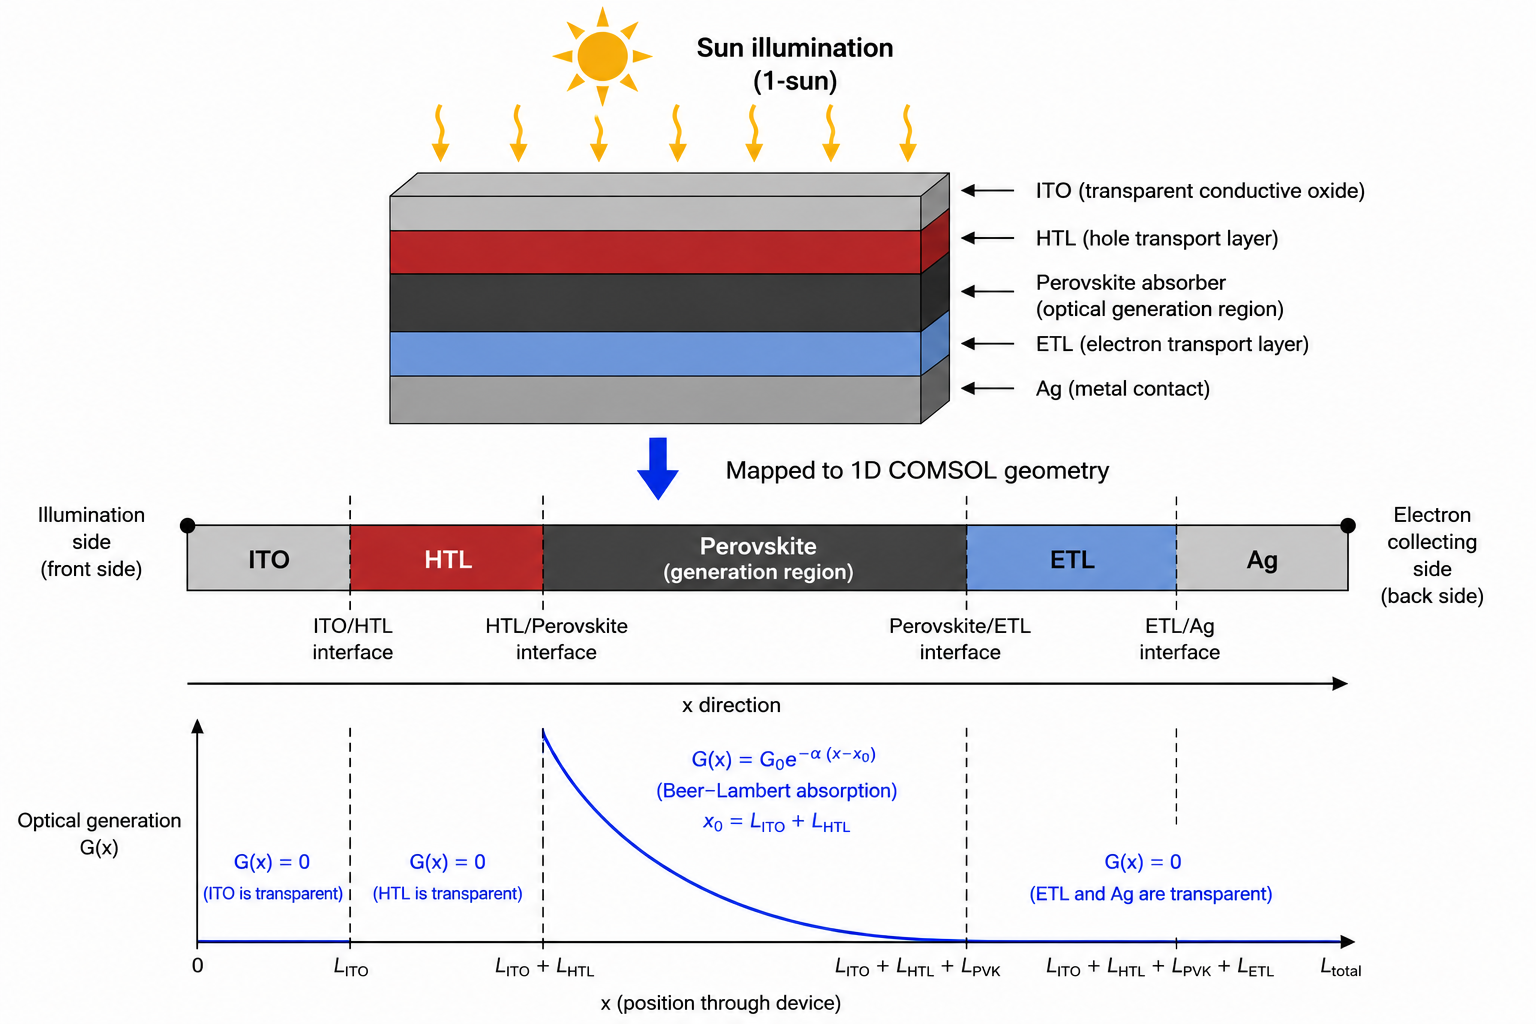
\includegraphics[width=0.96\textwidth]{figures/pptx_ai/psc_architecture_illumination_1d_mapping.png}
\caption{Laboratory p-i-n device architecture and its reduced 1-D COMSOL
mapping. Illumination enters from the ITO/HTL side, the transport layers and
absorber are mapped onto the model $x$ direction, and optical generation is
applied only in the perovskite absorber using the Beer--Lambert profile
implemented below.}
\label{fig:psc_stack_geometry}
\end{figure}

\section{Semiconductor Module Implementation}

The Semiconductor Module solves the coupled electronic transport problem by
assembling Poisson's equation, electron and hole continuity equations, and
current-density relations on the one-dimensional mesh \cite{comsol64}. Material
properties such as relative permittivity, mobility, band gap, electron affinity,
effective density of states, recombination lifetime, and trap density are
assigned by domain. For the laboratory architecture used here, the electrical
boundaries represent ITO at the illuminated side and Ag at the rear side. The target
coordinate convention is $x=0$ at ITO/HTL and increasing through the
perovskite toward ETL/Ag.

The primary dependent variables are the electrostatic potential and carrier
concentrations or quasi-Fermi-level variables, depending on the COMSOL
formulation selected in the model. The physical role is the same in either
formulation: COMSOL solves the nonlinear drift-diffusion system so that the
terminal current density is consistent with electrostatics, generation,
recombination, and boundary injection. The solver output is a simulated J--V
curve for the selected voltage protocol and internal state.

\begin{figure}[H]
\centering
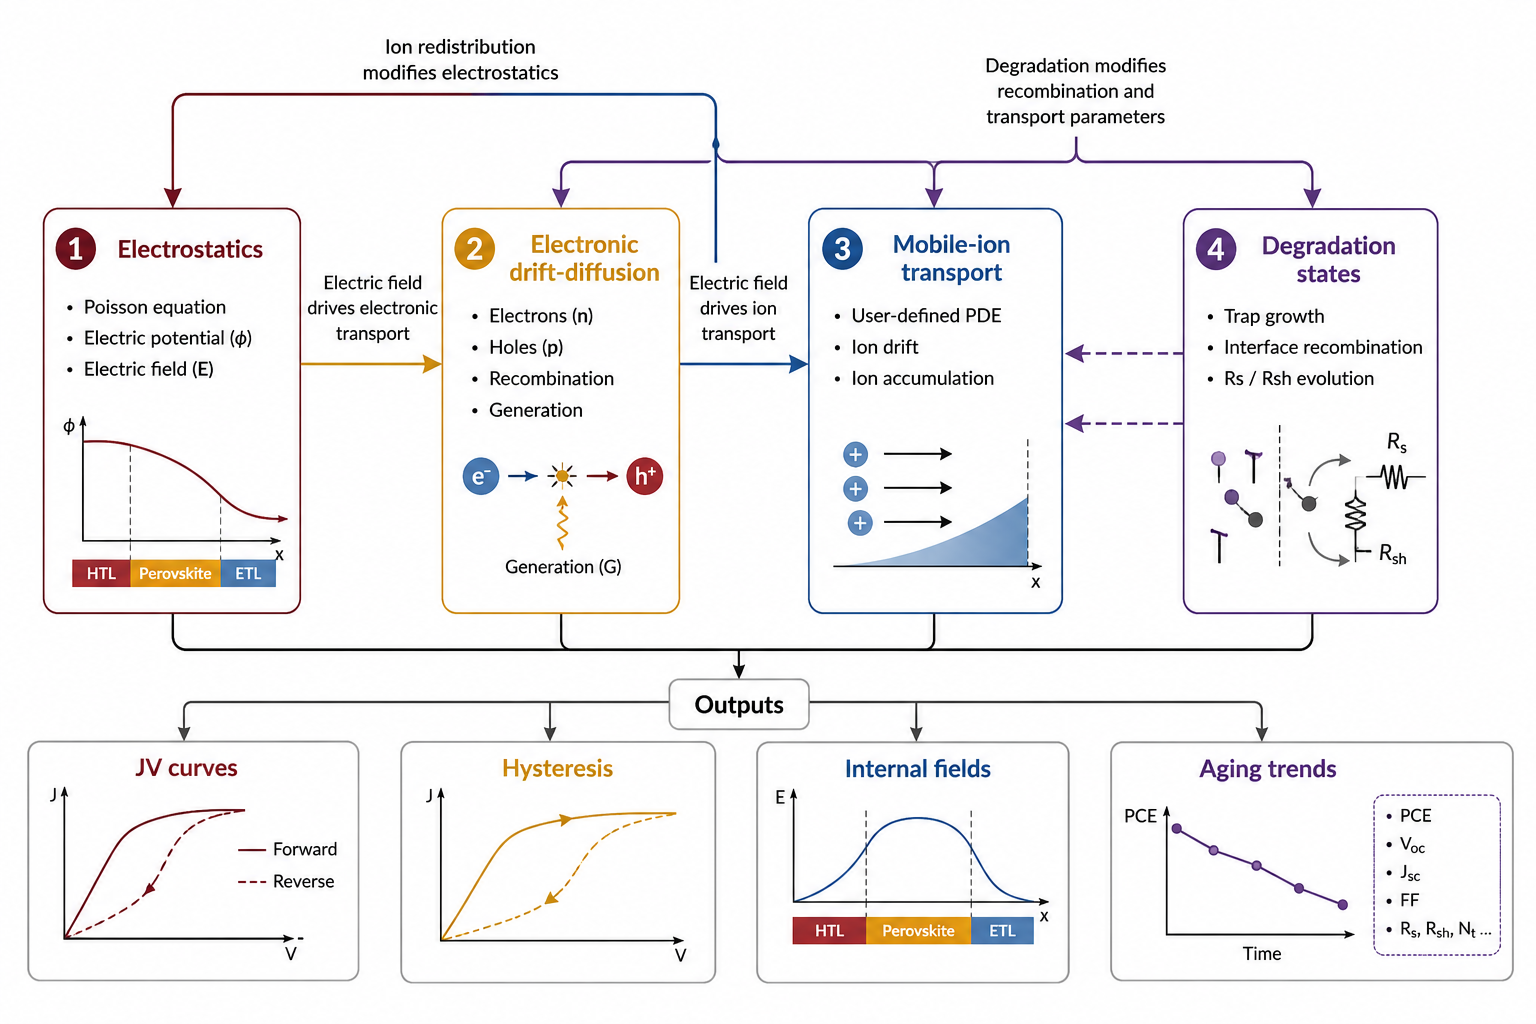
\includegraphics[width=\textwidth]{figures/pptx_ai/coupled_physics_workflow.png}
\caption{Coupled-physics structure of the COMSOL model. Electrostatics drives electronic transport and mobile-ion migration; ion redistribution feeds back through the electrostatic source term; degradation states modify recombination and transport parameters; the outputs include J--V curves, hysteresis, internal fields, and aging trends.}
\label{fig:coupled_physics_workflow}
\end{figure}

\section{Optical Generation Model}

The Semiconductor Module requires a volumetric electron-hole pair generation
rate in the perovskite absorber. The COMSOL implementation does not solve the
optical field with the Wave Optics interface. Optical absorption is represented
with an algebraic Beer--Lambert profile that is supplied directly to the
Semiconductor interface as a source term. The formulation is used in the
one-dimensional p-i-n stack
\begin{equation}
\mathrm{ITO}/(\mathrm{NiO}_x+\mathrm{MeO\mbox{-}2PACz})/
\mathrm{Cs}_{0.2}\mathrm{FA}_{0.8}\mathrm{PbI}_3/
(\mathrm{C}_{60}+\mathrm{BCP})/\mathrm{Ag},
\end{equation}
with active-layer dimensions
\begin{align}
\mathrm{thickness}_{\mathrm{ETL}} &= 29~\mathrm{nm},\\
\mathrm{thickness}_{\mathrm{PVK}} &= 450~\mathrm{nm},\\
\mathrm{thickness}_{\mathrm{HTL}} &= 35~\mathrm{nm},\\
A &= 9\times10^{-6}~\mathrm{m^2}.
\end{align}

The Beer--Lambert approximation assumes that the photon flux decays
exponentially through the absorber:
\begin{equation}
I(x)=I_0 e^{-\alpha_{\mathrm{pvk}}x_{\mathrm{pvk}}},
\end{equation}
where $I_0$ is the optical intensity entering the perovskite,
$\alpha_{\mathrm{pvk}}$ is the effective absorber absorption coefficient, and
$x_{\mathrm{pvk}}$ is the local depth measured from the illuminated
perovskite interface. The absorbed optical power density is
\begin{equation}
P_{\mathrm{abs}}(x_{\mathrm{pvk}})
=\alpha_{\mathrm{pvk}} I_0 e^{-\alpha_{\mathrm{pvk}}x_{\mathrm{pvk}}}.
\end{equation}
Using an effective photon energy
\begin{equation}
E_{\mathrm{ph}}=\frac{hc}{\lambda_{\mathrm{eff}}},
\end{equation}
the volumetric electron-hole pair generation rate becomes
\begin{equation}
G_{\mathrm{opt}}(x_{\mathrm{pvk}})
=\frac{\alpha_{\mathrm{pvk}}I_0\lambda_{\mathrm{eff}}}{hc}
e^{-\alpha_{\mathrm{pvk}}x_{\mathrm{pvk}}}.
\label{eq:beer_lambert_physical}
\end{equation}
This expression has units of m$^{-3}$s$^{-1}$ when $I_0$ is in W/m$^2$,
$\alpha_{\mathrm{pvk}}$ is in m$^{-1}$, and $\lambda_{\mathrm{eff}}$ is in m.
The direct COMSOL variable set for this physical form is
\texttt{alpha\_pvk}, \texttt{I0}, \texttt{lambda\_eff},
\texttt{Ephoton}, \texttt{x\_pvk}, and \texttt{Gopt}. The current model uses the
same Beer--Lambert depth dependence as a normalized algebraic shape so that
photogeneration can be calibrated independently from the front/back absorption
contrast.

The local perovskite coordinate is
\begin{equation}
x_{\mathrm{pvk}}=x-x_{\mathrm{pvk},0},
\end{equation}
with
\begin{equation}
x_{\mathrm{pvk},0}=\mathrm{thickness\_ETL},
\qquad
L_{\mathrm{gen}}=\mathrm{thickness\_PVK}.
\end{equation}
To avoid evaluating the exponential outside the perovskite domain, the local
coordinate is clipped:
\begin{equation}
x_{\mathrm{clip}}=
\min\left(\max\left(x_{\mathrm{pvk}},0\right),L_{\mathrm{gen}}\right).
\end{equation}

The raw dimensionless Beer--Lambert shape is
\begin{equation}
S_{\mathrm{raw}}(x)=e^{-\alpha_{\mathrm{gen}}x_{\mathrm{clip}}}.
\end{equation}
For numerical stability, COMSOL applies a small floor:
\begin{equation}
S_{\mathrm{raw}}(x)=
\max\left(e^{-\alpha_{\mathrm{gen}}x_{\mathrm{clip}}},
S_{\mathrm{floor}}\right).
\end{equation}
The analytical average of the unbounded exponential shape over the absorber is
\begin{equation}
\left\langle S_{\mathrm{raw}}\right\rangle =
\frac{1}{L_{\mathrm{gen}}}
\int_0^{L_{\mathrm{gen}}}e^{-\alpha_{\mathrm{gen}}x}\,dx,
\end{equation}
which gives
\begin{equation}
\left\langle S_{\mathrm{raw}}\right\rangle =
\frac{1-e^{-\alpha_{\mathrm{gen}}L_{\mathrm{gen}}}}
{\alpha_{\mathrm{gen}}L_{\mathrm{gen}}}.
\end{equation}
The normalized generation shape is
\begin{equation}
S_{\mathrm{norm}}(x)=
\frac{S_{\mathrm{raw}}(x)}
{\max\left(\left\langle S_{\mathrm{raw}}\right\rangle,
S_{\mathrm{floor}}\right)}.
\end{equation}
This normalization makes the spatial average of the shape approximately unity,
so the generation profile changes the depth distribution of photogeneration
without unintentionally changing the integrated generation strength.

The final optical generation rate is
\begin{equation}
G_{\mathrm{opt}}(x)=
G_0 S_{\mathrm{scale}}S_{\mathrm{norm}}(x).
\end{equation}
In the COMSOL variable set, this is implemented as
\begin{center}
\texttt{Gopt = G0\_0*Gshape\_scale*Gshape\_norm}.
\end{center}
The variables \texttt{Gshape\_raw}, \texttt{Gshape\_avg}, and \texttt{Gshape\_norm} are
dimensionless. \texttt{Gopt} has the same units as \texttt{G0\_0}, typically
1/(m$^3$s). If separate electron and hole generation fields are required by the
Semiconductor interface, both use the same algebraic expression,
\texttt{Gopt}. \texttt{Gopt} is not a solved dependent variable.

\begin{table}[H]
\centering
\footnotesize
\caption{COMSOL parameters for the algebraic Beer--Lambert generation profile.}
\label{tab:beer_lambert_parameters}
\begin{tabular}{p{0.20\textwidth}p{0.34\textwidth}p{0.36\textwidth}}
\toprule
Parameter & Expression & Meaning \\
\midrule
\texttt{alpha\_gen} & \texttt{5e6[1/m]} & Effective Beer--Lambert absorption coefficient \\
\texttt{Gshape\_floor} & \texttt{1e-6} & Numerical floor for the generation shape \\
\texttt{Gshape\_scale} & \texttt{1} & Manual generation calibration multiplier \\
\texttt{x\_pvk0} & \texttt{thickness\_ETL} & Start coordinate of the perovskite layer \\
\texttt{x\_pvk1} & \texttt{thickness\_ETL + thickness\_PVK} & End coordinate of the perovskite layer \\
\texttt{Lgen} & \texttt{thickness\_PVK} & Optical generation thickness \\
\bottomrule
\end{tabular}
\end{table}

\begin{table}[H]
\centering
\footnotesize
\caption{COMSOL variables for the normalized Beer--Lambert generation source.}
\label{tab:beer_lambert_variables}
\begin{tabular}{p{0.18\textwidth}p{0.48\textwidth}p{0.24\textwidth}}
\toprule
Variable & COMSOL expression & Meaning \\
\midrule
\texttt{xpvk} & \texttt{x-x\_pvk0} & Local coordinate into the perovskite \\
\texttt{xpvk\_clip} & \texttt{min(max(xpvk,0[m]),Lgen)} & Clipped local coordinate \\
\texttt{Gshape\_raw} &
\begin{tabular}[t]{@{}l@{}}
\texttt{max(exp(-alpha\_gen*xpvk\_clip),}\\
\texttt{Gshape\_floor)}
\end{tabular}
& Raw Beer--Lambert shape \\
\texttt{Gshape\_avg} &
\begin{tabular}[t]{@{}l@{}}
\texttt{(1-exp(-alpha\_gen*Lgen))/}\\
\texttt{(alpha\_gen*Lgen)}
\end{tabular}
& Analytical average of the exponential profile \\
\texttt{Gshape\_norm} &
\begin{tabular}[t]{@{}l@{}}
\texttt{Gshape\_raw/max(Gshape\_avg,}\\
\texttt{Gshape\_floor)}
\end{tabular}
& Normalized generation shape \\
\texttt{Gopt} & \texttt{G0\_0*Gshape\_scale*Gshape\_norm} & Final optical generation rate \\
\bottomrule
\end{tabular}
\end{table}

For \texttt{alpha\_gen = 5e6[1/m]} and
\texttt{Lgen = 450[nm]},
\begin{equation}
\alpha_{\mathrm{gen}}L_{\mathrm{gen}}
=5\times10^6 \times 450\times10^{-9}=2.25.
\end{equation}
The raw back/front generation ratio is therefore
\begin{equation}
e^{-2.25}\approx0.105.
\end{equation}
Before normalization, generation at the back of the absorber is about 10.5\%
of the generation near the illuminated side. For
\texttt{alpha\_gen = 1e7[1/m]},
\begin{equation}
\alpha_{\mathrm{gen}}L_{\mathrm{gen}}=4.5,
\end{equation}
and
\begin{equation}
e^{-4.5}\approx0.011.
\end{equation}
The profile is then much more front-loaded. The parameter
\texttt{alpha\_gen} is therefore treated as an effective
calibration/sensitivity parameter rather than a fully resolved optical
constant.

The generation profile should first be plotted over the perovskite domain to
confirm that it decreases monotonically from the illuminated side and remains
finite. The J--V curve should then be compared against the calibrated baseline
to evaluate changes in \texttt{Jsc}, \texttt{Voc}, \texttt{FF}, \texttt{PCE},
carrier-density profiles, recombination profiles, and local degradation
drivers.

\section{Mobile-Ion PDE}

Mobile ions are represented with a user-defined drift-diffusion equation,
consistent with mixed ionic-electronic PSC modeling practice
\cite{Richardson_2016,Calado_2022_Driftfusion}. For an ionic concentration
$c_{\mathrm{ion}}$, conservation gives
\begin{equation}
\frac{\partial c_{\mathrm{ion}}}{\partial t}
= -\nabla\cdot\mathbf{N}_{\mathrm{ion}},
\end{equation}
with Nernst--Planck flux
\begin{equation}
\mathbf{N}_{\mathrm{ion}}
= -D_{\mathrm{ion}}\nabla c_{\mathrm{ion}}
- \mu_{\mathrm{ion}} z_{\mathrm{ion}} q c_{\mathrm{ion}}\nabla\phi .
\label{eq:ion_flux}
\end{equation}
Here $D_{\mathrm{ion}}$ is ion diffusivity in m$^2$/s, $\mu_{\mathrm{ion}}$ is
ion mobility in m$^2$/(V s), $z_{\mathrm{ion}}$ is the signed ion valence, and
$\mathbf{N}_{\mathrm{ion}}$ has units of m$^{-2}$s$^{-1}$. Since
$\mathbf{E}=-\nabla\phi$, the migration term may also be written as
$\mu_{\mathrm{ion}} z_{\mathrm{ion}} q c_{\mathrm{ion}}\mathbf{E}$ depending
on sign convention. The implemented convention must match the sign of
$z_{\mathrm{ion}}$ and the direction of the electric field in COMSOL.

The dependent variable used in the General Form PDE interface is the normalized
ion state
\begin{equation}
u_{\mathrm{ion}}=\frac{c_{\mathrm{ion}}}{c_{\mathrm{ion},0}},
\qquad
c_{\mathrm{ion}}=c_{\mathrm{ion},0}u_{\mathrm{ion}},
\end{equation}
where $c_{\mathrm{ion},0}$ is the initial mobile-ion concentration. Substituting
into the conservation equation gives
\begin{equation}
\frac{\partial u_{\mathrm{ion}}}{\partial t}
=
\nabla\cdot\left[
D_{\mathrm{ion}}\nabla u_{\mathrm{ion}}
+ \mu_{\mathrm{ion}} z_{\mathrm{ion}} q u_{\mathrm{ion}}\nabla\phi
\right].
\label{eq:normalized_ion}
\end{equation}
The normalized state is dimensionless, so each term in
Eq.~\ref{eq:normalized_ion} has units of 1/s. In COMSOL, this equation is
implemented in the perovskite domain using the electrostatic potential from the
Semiconductor Module as a coupled field.

For one-dimensional implementation and diagnostics, it is useful to write the
normalized ion flux in terms of the electric field used to drive migration:
\begin{equation}
\Gamma_u
=-\frac{\partial u_{\mathrm{ion}}}{\partial x}
+\frac{z_{\mathrm{ion}}q}{k_{\mathrm{B}}T}
u_{\mathrm{ion}}E_{\mathrm{ion}} .
\label{eq:normalized_ion_flux}
\end{equation}
Here $E_{\mathrm{ion}}$ is the actual field supplied to the ion equation in
V/m. The corresponding physical particle flux and ionic current density are
\begin{align}
N_{\mathrm{ion}} &=D_{\mathrm{ion}}c_{\mathrm{ion},0}\Gamma_u,\\
J_{\mathrm{ion}} &=z_{\mathrm{ion}}qN_{\mathrm{ion}} .
\end{align}
These forms provide direct unit checks: $N_{\mathrm{ion}}$ has units
m$^{-2}$s$^{-1}$ and $J_{\mathrm{ion}}$ has units A/m$^2$.

The ionic charge density coupled into Poisson electrostatics is
\begin{equation}
\rho_{\mathrm{ion}}
=
\gamma_{\mathrm{ion}} q z_{\mathrm{ion}} c_{\mathrm{ion},0}
\left(u_{\mathrm{ion}}-1\right).
\label{eq:rho_ion}
\end{equation}
The factor $\gamma_{\mathrm{ion}}$ is a scaling or participation factor used to
control how strongly the normalized ion redistribution perturbs electrostatics.
The term $(u_{\mathrm{ion}}-1)$ is used so that a spatially uniform initial ion
distribution does not create artificial net space charge. Only redistribution
away from the initial uniform state contributes to the electrostatic source
term. The default ion boundary condition is blocking flux at the perovskite
interfaces unless an interfacial exchange model is explicitly specified.

\section{Mobile-Ion Preconditioning}

Perovskite devices do not enter a J--V scan from a unique uniform ionic state.
Bias history, illumination, and rest conditions redistribute mobile defects
before the measurement begins, and that ionic profile can screen or reinforce
the internal field during the subsequent voltage protocol
\cite{Eames_2015,Richardson_2016,Calado_2016}. The COMSOL workflow therefore
treats ion preconditioning as part of the initial condition rather than as a
post-processing correction.

The preconditioning sequence is:
\begin{enumerate}
\item solve the electronic stack at the selected dark or illuminated operating
condition;
\item run a time-dependent ion-relaxation study at the chosen history voltage
or open-circuit condition;
\item use the final $u_{\mathrm{ion}}(x,t_{\mathrm{pre}})$ distribution as the
initial condition for the J--V, hysteresis, or DIT study; and
\item verify ion conservation by checking that the absorber average of
$u_{\mathrm{ion}}$ remains close to unity.
\end{enumerate}
The same check should also inspect the maximum and minimum values of
$u_{\mathrm{ion}}$, the interfacial flux, and the resulting
$\rho_{\mathrm{ion}}$ profile. Large boundary spikes often indicate that the
field scaling, mesh, time stepping, or blocking boundary condition is forcing
an unphysical double layer.

In the COMSOL implementation, the electric-field expression supplied to the
ion equation must be consistent with the plotted electrostatic potential. The
symbolic derivative \texttt{d(V,x)} can evaluate to zero or to an unintended
field if the selected dependent variable is not the Semiconductor Module
potential. The Semiconductor Module field component, \texttt{semi.Ex}, is the
preferred diagnostic because it is consistent with the potential slope plotted
from the solved semiconductor physics. When additional numerical stabilization
or applied-bias control is needed, the ion-driving field is written as
\begin{equation}
E_{\mathrm{ion}}
=\eta_{E,\mathrm{bi}}E_{\mathrm{semi},x}
+\eta_{\mathrm{app}}\frac{V_{\mathrm{drive}}}{L_{\mathrm{pvk}}},
\end{equation}
where $E_{\mathrm{semi},x}$ is taken from \texttt{semi.Ex},
$L_{\mathrm{pvk}}$ is the perovskite thickness, and the dimensionless
$\eta$ factors are calibration and stabilization factors. For a 500 nm
absorber, a field of $10^6$ V/m corresponds to a 0.5 V potential drop, while
$k_{\mathrm{B}}T/q$ is only about 25.9 mV at room temperature. Unscaled fields
can therefore imply very large Boltzmann concentration ratios. Practical
preconditioning studies require bounded ion variables, conservative flux
settings, mesh refinement near interfaces, and comparison against
ion-sensitive measurements before the extracted ion concentration is treated
as unique.

\section{Stress-Dependent Mobile-Ion Transport and Degradation Coupling}

The mobile-ion model is extended from a static degradation-parameter
description into a dynamic stress-dependent formulation. Mobile-ion
redistribution is treated as a reversible, or partially reversible,
fast-to-medium-time-scale process. Material degradation is treated as a slower
irreversible process driven by stressors such as heat, illumination, electric
field, and local ion accumulation. This separation is important for calibration:
the model should first reproduce mobile-ion transport, then add one
degradation channel at a time. The first irreversible channel used for model
development is trap-density growth because it couples directly to SRH
recombination and therefore affects $V_{oc}$, FF, and PCE.

\subsection{Temperature and Light Dependence}

Mobile-ion diffusivity is thermally activated in hybrid lead iodide
perovskites, with iodide-related vacancy migration often treated as a dominant
fast ionic pathway \cite{Eames_2015,Futscher_2019}. The diffusivity is written
relative to a reference value:
\begin{equation}
D_{\mathrm{ion}}(T)
=D_{\mathrm{ion,ref}}
\exp\left[
-\frac{E_{a,\mathrm{ion}}}{k_{\mathrm{B}}}
\left(\frac{1}{T}-\frac{1}{T_{\mathrm{ref}}}\right)
\right].
\end{equation}
When the activation energy is entered in electron-volts, the COMSOL expression
uses $k_{\mathrm{B,eV}}=8.617333262\times10^{-5}$ eV/K:
\begin{equation}
D_{\mathrm{ion},T}
=D_{\mathrm{ion,ref}}
\exp\left[
-\frac{E_{a,\mathrm{ion}}}{k_{\mathrm{B,eV}}}
\left(\frac{1}{T_{\mathrm{dev}}}-\frac{1}{T_{\mathrm{ref}}}\right)
\right].
\label{eq:dion_temperature}
\end{equation}
In COMSOL notation, the corresponding parameters are
\texttt{Tdev}, \texttt{Tref}, \texttt{Ea\_Dion}, \texttt{kB\_eV},
\texttt{Dion\_ref}, and
\begin{center}
\texttt{Dion\_T = Dion\_ref*exp(-(Ea\_Dion/kB\_eV)*(1/Tdev - 1/Tref))}.
\end{center}
The constant diffusivity in the ion PDE is then replaced by
\texttt{Dion\_T}. The same temperature must also be used in the drift term:
\begin{equation}
\Gamma_u
=-\frac{\partial u_{\mathrm{ion}}}{\partial x}
+\frac{z_{\mathrm{ion}}q}{k_{\mathrm{B}}T_{\mathrm{dev}}}
u_{\mathrm{ion}}E_{\mathrm{ion}}.
\label{eq:gamma_tdev}
\end{equation}
Increasing temperature therefore accelerates ion kinetics through
$D_{\mathrm{ion},T}$, but also increases the thermal voltage
$k_{\mathrm{B}}T/q$. For a fixed electric field, the higher thermal voltage
can reduce the equilibrium concentration contrast even while the approach to
that equilibrium becomes faster.

Illumination can also affect ion motion through photogenerated carriers,
photovoltage, trap occupation, defect chemistry, and field screening
\cite{Calado_2016,Calado_2022_Driftfusion}. Because the microscopic route is
device dependent, the first implementation treats light as a controlled
phenomenological multiplier on diffusivity rather than as a change in total
mobile-ion inventory. Starting from the Beer--Lambert generation in
Eq.~\ref{eq:beer_lambert_physical}, the perovskite-average generation is
normalized as
\begin{equation}
G_{\mathrm{norm}}=
\frac{\langle G_{\mathrm{opt}}\rangle_{\mathrm{pvk}}}
{G_{\mathrm{1sun,ref}}},
\end{equation}
and the ion-transport multiplier is
\begin{align}
f_{\mathrm{light,ion}} &=
1+A_{\mathrm{light,ion}}G_{\mathrm{norm}}^{m_{\mathrm{light,ion}}},\\
D_{\mathrm{ion,eff}} &= D_{\mathrm{ion},T}f_{\mathrm{light,ion}}.
\label{eq:dion_eff}
\end{align}
The COMSOL variables are \texttt{Gavg\_pvk}, \texttt{Gnorm},
\texttt{A\_light\_ion}, \texttt{m\_light\_ion}, \texttt{flight\_ion}, and
\texttt{Dion\_eff}. The dark-validation value is
\texttt{A\_light\_ion = 0}. Only after dark ion transport is stable should this
coefficient be increased for sensitivity testing. The inventory
\texttt{cion0} remains the conserved total mobile-ion concentration unless DIT
or aging data justify a separate light-activated ion-creation state.

\subsection{Electric-Field Driving and History Dependence}

Voltage dependence enters the ion equation through the Nernst--Planck drift
term. With $u_{\mathrm{ion}}=c_{\mathrm{ion}}/c_{\mathrm{ion},0}$,
\begin{align}
N_{\mathrm{ion},x} &= D_{\mathrm{ion,eff}}c_{\mathrm{ion},0}\Gamma_u,\\
J_{\mathrm{ion},x} &= z_{\mathrm{ion}}qN_{\mathrm{ion},x}.
\end{align}
The field used in $\Gamma_u$ must be the actual field supplied to the ion PDE.
In the present Semiconductor implementation, directly using
\texttt{d(V,x)} was not reliable because it could evaluate to zero even when
the plotted electrostatic potential had a visible slope. The Semiconductor
field variable \texttt{semi.Ex} captured the physically consistent field. The
ion-driving field is therefore written as
\begin{equation}
E_{\mathrm{ion}}=\eta_E E_{\mathrm{semi},x},
\end{equation}
or, for protocols where the applied voltage must be controlled separately,
\begin{equation}
E_{\mathrm{ion}}
=\eta_{E,\mathrm{bi}}E_{\mathrm{semi},x}
+\eta_{\mathrm{app}}\frac{V_{\mathrm{drive}}}{L_{\mathrm{pvk}}}.
\label{eq:eion_scaled}
\end{equation}
The scaling factors are numerical and physical safeguards. The full
semiconductor field can overdrive the ion PDE and produce unphysical
interfacial pileup. A field of $10^6$ V/m across 500 nm corresponds to about
0.5 V, while $k_{\mathrm{B}}T/q\approx25.9$ mV at 300 K; an unrestricted
Boltzmann ratio $\exp(qV/k_{\mathrm{B}}T)$ can therefore become extremely
large. Field scaling, concentration floors and caps, mesh refinement, and
ion-conservation checks keep the model interpretable. With the sign convention
in Eq.~\ref{eq:gamma_tdev}, a positive mobile iodide vacancy has
$z_{\mathrm{ion}}=+1$. If \texttt{semi.Ex} is negative, positive ions drift
toward negative $x$, matching the left-interface accumulation observed after
the field sign was corrected.

History dependence is implemented through preconditioning rather than by
assuming $u_{\mathrm{ion}}=1$ at every measurement. The workflow solves the
electronic initial state, relaxes the ion PDE under a selected rest, bias,
light-soak, open-circuit, short-circuit, or MPP condition, stores
$u_{\mathrm{ion}}(x,t_{\mathrm{pre}})$, and uses that profile to initialize
J--V, hysteresis, DIT, or aging studies. A representative preconditioning case
produces a controlled interfacial accumulation profile: $\max(u_{\mathrm{ion}})$
increases from near 1 to approximately 30--40 over a 20 s simulation, with a
bulk region near $u_{\mathrm{ion}}\approx1$ and depletion near the opposite
interface. Keeping $\max(u_{\mathrm{ion}})$ near 20--30 represents a
moderate-to-strong ionic memory state suitable for measurable hysteresis or DIT
response. Blocking-boundary validation requires
$\langle u_{\mathrm{ion}}\rangle_{\mathrm{pvk}}\approx1$, nonnegative
$u_{\mathrm{ion}}$ above the imposed floor, mesh-resolved accumulation layers,
bounded maxima, and a flux that approaches a quasi-steady value during
preconditioning.

\subsection{Irreversible Trap-Growth Coupling}

The slower degradation model introduces dimensionless bounded states
$D_{\mathrm{trap}}$, $D_{\mathrm{interface}}$, $D_{Rs}$, and $D_{Rsh}$. These
states are severity coordinates, not directly measured concentrations. The
staged implementation begins with trap growth:
\begin{equation}
\frac{\partial D_{\mathrm{trap}}}{\partial t}
=k_{\mathrm{trap}}(T)
f_{\mathrm{light,deg}}f_{\mathrm{field,deg}}f_{\mathrm{ion,deg}}
\left(1-D_{\mathrm{trap}}\right),
\label{eq:dtrap_stress}
\end{equation}
where
\begin{equation}
k_{\mathrm{trap}}(T)
=k_{\mathrm{trap,ref}}
\exp\left[
-\frac{E_{a,\mathrm{trap}}}{k_{\mathrm{B,eV}}}
\left(\frac{1}{T_{\mathrm{dev}}}-\frac{1}{T_{\mathrm{ref}}}\right)
\right].
\end{equation}
The stress multipliers may be written as
\begin{align}
f_{\mathrm{light,deg}} &=
1+A_{L,\mathrm{deg}}G_{\mathrm{norm}}^{m_{L,\mathrm{deg}}},\\
f_{\mathrm{field,deg}} &=
1+A_{E,\mathrm{deg}}
\left(\frac{E_{\mathrm{stress}}}{E_{\mathrm{ref}}}\right)^{m_{E,\mathrm{deg}}},\\
f_{\mathrm{ion,deg}} &=
1+A_{\mathrm{ion,deg}}
\left(\frac{\mathrm{ion}_{\mathrm{accum}}}{\mathrm{ion}_{\mathrm{ref}}}\right)^{m_{\mathrm{ion,deg}}}.
\end{align}
Suitable stress metrics are the average or maximum of $|E_{\mathrm{ion}}|$ in
the perovskite, $\max(u_{\mathrm{ion}})-1$, an interface average of
$u_{\mathrm{ion}}-1$, and $G_{\mathrm{norm}}$. Trap damage then enters the
Semiconductor Module through
\begin{equation}
N_{t,\mathrm{eff}}=N_{t0}\left(1+A_{Nt,\mathrm{deg}}D_{\mathrm{trap}}\right).
\end{equation}
This is the first degradation channel because it is physically plausible under
ion accumulation, heat, light, and field stress; it has a direct SRH
recombination pathway; and it can be debugged before multiple loss channels
are allowed to compensate one another. Future channels can use
\begin{align}
S_{\mathrm{eff}} &= S_0\left(1+A_{S,\mathrm{deg}}D_{\mathrm{interface}}\right),\\
R_{s,\mathrm{eff}} &= R_{s0}\left(1+A_{Rs,\mathrm{deg}}D_{Rs}\right),\\
R_{sh,\mathrm{eff}} &= \frac{R_{sh0}}{1+A_{Rsh,\mathrm{deg}}D_{Rsh}},
\end{align}
but they should not be activated as calibrated physics until each individual
channel has been tested against mechanism-specific observables.

\begin{table}[H]
\centering
\scriptsize
\caption{Core variables for stress-dependent ion transport and staged degradation coupling.}
\label{tab:stress_dependent_ion_variables}
\begin{tabular}{@{}p{0.16\textwidth}p{0.31\textwidth}p{0.13\textwidth}p{0.25\textwidth}@{}}
\toprule
Variable & Meaning & Units & Role \\
\midrule
\texttt{Tdev} & Device temperature & K & Sets diffusivity and thermal voltage \\
\texttt{Dion\_T} & Arrhenius ion diffusivity & m$^2$/s & Temperature-dependent ion kinetics \\
\texttt{Dion\_eff} & Effective ion diffusivity & m$^2$/s & Includes temperature and optional light multiplier \\
\texttt{Gnorm} & Normalized perovskite generation & 1 & Light-stress metric \\
\texttt{Eion} & Ion-driving electric field & V/m & Drift term in the ion PDE \\
\texttt{eta\_E}, \texttt{eta\_app} & Field-scaling factors & 1 & Stabilize and calibrate field coupling \\
\texttt{uion} & Normalized mobile-ion state & 1 & Reversible ionic memory variable \\
\texttt{cion0} & Total mobile-ion inventory & m$^{-3}$ or cm$^{-3}$ & Conserved baseline concentration \\
\texttt{D\_trap} & Trap-damage severity & 1 & First irreversible degradation state \\
\texttt{Nt\_eff} & Effective trap density & m$^{-3}$ or cm$^{-3}$ & Semiconductor recombination input \\
\bottomrule
\end{tabular}
\end{table}

\begin{table}[H]
\centering
\footnotesize
\caption{Staged roadmap for stress-dependent mobile-ion and degradation model development.}
\label{tab:stress_dependent_model_roadmap}
\begin{tabular}{p{0.16\textwidth}p{0.36\textwidth}p{0.38\textwidth}}
\toprule
Stage & Model addition & Validation target \\
\midrule
1 & Temperature-dependent ion diffusivity & Max/min/average $u_{\mathrm{ion}}$ versus time at 300, 330, and 360 K \\
2 & Light-dependent ion-mobility factor & Dark versus 1-sun preconditioning and DIT response \\
3 & Field-driven migration using \texttt{semi.Ex} and \texttt{Vdrive} & Scan-rate-dependent J--V hysteresis and DIT pulse response \\
4 & Trap-degradation state $D_{\mathrm{trap}}$ & $N_{t,\mathrm{eff}}$ increases under light/heat/field/ion stress; $V_{oc}$, FF, and PCE degrade consistently \\
5 & Additional $D_{\mathrm{interface}}$, $D_{Rs}$, and $D_{Rsh}$ channels & Mechanism-specific J--V signatures before full-channel coupling \\
\bottomrule
\end{tabular}
\end{table}

The constants used by this section are the elementary charge $q$, Boltzmann
constant $k_{\mathrm{B}}$, $k_{\mathrm{B,eV}}=8.617333262\times10^{-5}$ eV/K,
Planck constant $h$, speed of light $c$, and reference temperature
$T_{\mathrm{ref}}$, typically 300 K. The thermal voltage is
$k_{\mathrm{B}}T/q\approx25.9$ mV at 300 K.

\section{Known Protocols and Hidden States}

The COMSOL hysteresis workflow separates measurement protocol from device
state. The known inputs are quantities controlled or directly measured during a
scan:
\begin{equation}
\mathbf{u}(t) =
\left[V(t), \dot{V}(t), r_{\mathrm{scan}}, V_{\min}, V_{\max},
t_{\mathrm{pre}}, t_{\mathrm{rest}}\right].
\end{equation}
The hidden or model-internal quantities are material and device states:
\begin{equation}
\boldsymbol{\theta} =
\left[R_s, R_{sh}, c_{\mathrm{ion},0}, D_{\mathrm{ion}},
N_t, Q_f, S, G_{\mathrm{eff}}, \ldots\right].
\end{equation}
Scan rate is known because the experimenter sets it. Ion concentration,
diffusivity, trap density, interfacial charge, and resistance states are not
known from a terminal J--V measurement and must be represented as model
variables to be calibrated.

\section{J--V Metric Extraction}

The simulated terminal J--V curve is converted into standard photovoltaic
metrics after each voltage sweep. The short-circuit current density is
\begin{equation}
J_{sc}=J(V=0),
\end{equation}
and the open-circuit voltage satisfies
\begin{equation}
J(V_{oc})=0.
\end{equation}
If $V=0$ or $J=0$ is not exactly sampled, the value is obtained by interpolation
between neighboring simulated voltage points. The electrical power density is
\begin{equation}
P(V)=VJ(V),
\end{equation}
and the maximum-power point is
\begin{equation}
P_{\max}=V_{mpp}J_{mpp}.
\end{equation}
The fill factor and PCE are then
\begin{align}
\mathrm{FF} &=
\frac{V_{mpp}J_{mpp}}{V_{oc}J_{sc}},\\
\mathrm{PCE} &=
\frac{V_{mpp}J_{mpp}}{P_{\mathrm{in}}}.
\end{align}
The sign convention must be handled consistently because photovoltaic current
is often plotted with the power-generating quadrant inverted. In the processing
workflow, the MPP is selected from the power-producing branch of the simulated
J--V curve after applying the repository's current-density sign convention.

\section{COMSOL Quality Checks}

Each major model component is evaluated through a physical and numerical
checklist:
\begin{enumerate}
\item voltage, current-density, charge-density, and area-normalization units
must be consistent;
\item all-off controls must remain flat during degradation studies;
\item one-mechanism studies must produce the expected J--V signature;
\item coupled cases must be compared against one-mechanism and leave-one-out
cases to detect non-additive behavior;
\item selected cases must be checked under mesh and time-step refinement; and
\item simulated J--V, hysteresis, and aging trends must be compared against
matched laboratory measurements before device-specific claims are made.
\end{enumerate}
